\documentclass[12pt, a4paper, oneside]{Thesis} % Paper size, default font size and one-sided paper
\usepackage{wrapfig}
\usepackage{lscape}
\usepackage{lineno}
\modulolinenumbers[5]

\usepackage{array}
\usepackage{float}
\usepackage{placeins}
\usepackage{stackengine}
\usepackage{numprint}
\usepackage{siunitx}
%\usepackage[showframe=false]{geometry}

\nprounddigits{3}
\emergencystretch=1em
\newcolumntype{P}[1]{>{\centering\arraybackslash}p{#1}}
\newcolumntype{M}[1]{>{\centering\arraybackslash}m{#1}}

\setstackEOL{\#}
\setstackgap{L}{12pt}


%\usepackage{subcaption} %incompatible with subfig
\graphicspath{{Pictures/}} % Specifies the directory where pictures are stored
\usepackage[numbers]{natbib} % Use the natbib reference package - read up on this to edit the reference style; if you want text (e.g. Smith et al., 2012) for the in-text references (instead of numbers), remove 'numbers'

\hypersetup{urlcolor=black, colorlinks=false} % Colors hyperlinks in blue - change to black if annoying

\thesistitle{Live Code Interview Platform}
\supervisor{\shortstack{Dr. Amit Kumar Khaskalam }}
\degree{Bachelor of Technology}
\degreemajor{Information Technology, 6th Sem}
\authors{Brijesh kumar, Narendra, Suraj Biswas}
\rollno{23036115, 23036134, 23036168}
\university{Guru Ghasidas Vishwavidyalaya}
\department{Department of Information Technology}
\unisite{http://www.ggu.ac.in}
\depsite{https://www.ggu.ac.in/Department-Details.aspx?Id=MTY=}
\placeshrt{Bilaspur}
\placelng{Bilaspur - 495009, India}
\datesub{December 23, 2026}
\datesig{December 23, 2026}
\semsub{}
\keywords{XXXXXXXXXXX}
\coursecd{Project (ITUFPV1) Report}

\title{\ttitle} % Defines the thesis title - don't touch this
\begin{document}
%\makeatletter
%\renewcommand*{\NAT@nmfmt}[1]{\textsc{#1}}
%\makeatother

% prints author names as small caps


\frontmatter % Use roman page numbering style (i, ii, iii, iv...) for the pre-content pages

\setstretch{1.6} % Line spacing of 1.6 (double line spacing)

% Define the page headers using the FancyHdr package and set up for one-sided printing
\fancyhead{} % Clears all page headers and footers
\rhead{\thepage} % Sets the right side header to show the page number
\lhead{} % Clears the left side page header

\pagestyle{plain} % Use plain page style for frontmatter pages prior to Contents

\newcommand{\HRule}{\rule{\linewidth}{0.5mm}} % New command to make the lines in the title page

% PDF meta-data
\hypersetup{pdftitle={\ttitle}}
\hypersetup{pdfsubject=\subjectname}
\hypersetup{pdfauthor=\authornames}
\hypersetup{pdfkeywords=\keywordnames}

%----------------------------------------------------------------------------------------
%	TITLE PAGE
%----------------------------------------------------------------------------------------
\maketitle
%\titlepg % Add a gap in the Contents, for aesthetics

\clearpage % Start a new page

%----------------------------------------------------------------------------------------
%	DECLARATION PAGE
%	Your institution may give you a different text to place here
%----------------------------------------------------------------------------------------


\Declaration{} % Add a gap in the Contents, for aesthetics


%----------------------------------------------------------------------------------------
%	CERTIFICATE PAGE
%----------------------------------------------------------------------------------------

\addtotoc{Certificate} % Add the "Abstract" page entry to the Contents

\certificate{\addtocontents{toc}{}} % Add a gap in the Contents, for aesthetics

\clearpage % Start a new page

%----------------------------------------------------------------------------------------
%	ABSTRACT PAGE
%----------------------------------------------------------------------------------------

\addtotoc{Abstract} % Add the "Abstract" page entry to the Contents

\abstract{\addtocontents{toc}{} % Add a gap in the Contents, for aesthetics

}

\clearpage % Start a new page



%----------------------------------------------------------------------------------------
%	ACKNOWLEDGEMENTS
%----------------------------------------------------------------------------------------

\setstretch{1.7} % Reset the line-spacing to 1.3 for body text (if it has changed)

\acknowledgements{\addtocontents{toc}{}%\vspace{1em}} % Add a gap in the Contents, for aesthetics

We express our sincere gratitude to \textbf{Dr. Amit Kumar Khaskalam}, Associate Professor, Department of Information Technology, who served as the \textbf{Project Guide} for this project. We are deeply thankful for his valuable guidance, continuous encouragement, constructive suggestions, and constant supervision throughout the course of this work.

We would like to express our sincere thanks to the \textbf{Project In-Charge}, \textbf{Mr. Deepak Kant Netam}, Assistant Professor, Department of Information Technology, for his guidance, coordination, and support during the execution of this mini project.

We would also like to express our heartfelt gratitude to the Head of the Department of Information Technology, \textbf{Dr. Manoj Kumar}, for his leadership, motivation, and for providing the necessary academic support and resources during the development of this project.

We are extremely thankful to \textbf{Prof. M. Chakradhara Rao}, Dean, School of Studies in Engineering and Technology, Guru Ghasidas Vishwavidyalaya, for providing the required infrastructural facilities and a conducive academic environment, without which this work would not have been possible.

We also wish to extend our sincere thanks to the faculty members of the Department of Information Technology and our classmates for their inspiration, encouragement, insightful comments, and constructive suggestions, which helped in improving the quality of this project work.



}
\clearpage % Start a new page

%----------------------------------------------------------------------------------------
%	LIST OF CONTENTS/FIGURES/TABLES PAGES
%----------------------------------------------------------------------------------------

\pagestyle{fancy} % The page style headers have been "empty" all this time, now use the "fancy" headers as defined before to bring them back

\lhead{\emph{Contents}} % Set the left side page header to "Contents"
\tableofcontents % Write out the Table of Contents

\lhead{\emph{List of Figures}} % Set the left side page header to "List of Figures"
\listoffigures % Write out the List of Figures

%----------------------------------------------------------------------------------------
%	ABBREVIATIONS
%----------------------------------------------------------------------------------------


%----------------------------------------------------------------------------------------
%	PHYSICAL CONSTANTS/OTHER DEFINITIONS
%----------------------------------------------------------------------------------------
%
%\clearpage % Start a new page
%
%\lhead{\emph{Physical Constants}} % Set the left side page header to "Physical Constants"
%
%\listofconstants{lrcl} % Include a list of Physical Constants (a four column table)
%{
%Speed of Light & $c$ & $=$ & $2.997\ 924\ 58\times10^{8}\ \mbox{ms}^{-\mbox{s}}$ (exact)\\
%% Constant Name & Symbol & = & Constant Value (with units) \\
%}

%----------------------------------------------------------------------------------------
%	SYMBOLS
%----------------------------------------------------------------------------------------





%----------------------------------------------------------------------------------------
%	DEDICATION
%----------------------------------------------------------------------------------------
%
%\setstretch{1.3} % Return the line spacing back to 1.3
%
%\pagestyle{empty} % Page style needs to be empty for this page
%
%\dedicatory{For/Dedicated to/To my\ldots} % Dedication text
%
%\addtocontents{toc}{\vspace{2em}} % Add a gap in the Contents, for aesthetics

%----------------------------------------------------------------------------------------
%	THESIS CONTENT - CHAPTERS
%----------------------------------------------------------------------------------------

\mainmatter % Begin numeric (1,2,3...) page numbering

\pagestyle{fancy} % Return the page headers back to the "fancy" style

% Include the chapters of the thesis as separate files from the Chapters folder
% Uncomment the lines as you write the chapters

% Chapter 1: Introduction
\chapter{Introduction}
\label{Chapter1}
\lhead{Chapter 1. \emph{Introduction}}

In the contemporary digital landscape, personal productivity, mental health, and lifestyle optimization have emerged as paramount concerns. The widespread adoption of smart devices and digital trackers has spurred the growth of the ``Quantified-Self'' movement---an empirical paradigm where individuals continuously log behavioral, physiological, and psychological metrics to gain actionable self-knowledge. However, despite the abundance of specialized software applications, users face significant systemic fragmentation. Qualitative reflections (such as daily diary writing and mood tracking) are fundamentally decoupled from quantitative routines (such as sleep monitoring, screen time tracking, study sessions, and habit consistency). 

Modern users frequently employ multiple disjointed applications to track their daily lives: dedicated note-taking tools for journaling, separate habit trackers for recurring rituals, specialized affect apps for mood logs, and standalone timers or spreadsheets for study and financial records. These isolated repositories of personal data create telemetry silos. Crucially, disjointed architectures cannot perform cross-domain correlation. They fail to address vital multidimensional lifestyle questions, such as the direct empirical impact of inadequate sleep on daily emotional valence, the statistical influence of habitual exercise on career satisfaction, or the weekly cyclicality of psychological stress.

Furthermore, traditional self-tracking tools suffer from severe retrospective bias and cognitive friction. Most mobile trackers permit arbitrary historical backfilling, allowing individuals to retroactively log or falsify entries days later to maintain artificial streaks. This historical revisionism distorts longitudinal datasets and degrades the validity of any analytical inference. Concurrently, switching between multiple single-purpose applications imposes high cognitive load, causing a vast majority of users to abandon tracking within a few weeks.

To overcome these structural limitations, this project presents \textbf{ManologAI}---an engineering-grade, privacy-first personal life analytics platform and behavioral insight engine. Designed specifically to resolve the fragmented Quantified-Self problem, ManologAI unites qualitative daily reflections and an 8-scale quantized emotion tracking system with quantitative lifestyle metrics (sleep duration, screen time, study hours, habits, daily expenses, and weekly timetables) into a single cohesive, high-performance data pipeline. 

Rather than relying on non-deterministic generative models that are susceptible to analytical hallucination and opaque inference, ManologAI incorporates a deterministic behavioral intelligence engine based on statistical regression. By computing Pearson correlation coefficients ($r$) across sliding temporal windows and conducting empirical counterfactual baseline analyses ($\Delta$), ManologAI transforms raw chronological logs into objective, explainable, and natural-language diagnostic feedback. To ensure pristine historical datasets, the platform enforces a strict 24-hour temporal integrity lock via API middleware, precluding future logging and retroactive falsification. Built as a responsive Progressive Web App (PWA) with native RFC 8291/8292 VAPID push notifications, ManologAI delivers a frictionless sub-two-minute daily logging ritual, robust data integrity, and actionable personal intelligence for lifestyle optimization.

\section{Aim \& Objectives}

The primary aim of this project is to design, implement, and evaluate \textbf{ManologAI}, a comprehensive personal life analytics platform and deterministic behavioral insight engine that unifies qualitative and quantitative behavioral telemetry within an ergonomic, secure, and privacy-first full-stack environment.

The specific objectives of this project are:
\begin{itemize}
  \item To architect and develop a responsive, cross-platform Progressive Web App (PWA) using React 19, Vite, and Tailwind CSS that enables a comprehensive daily check-in ritual in under two minutes.
  \item To construct a high-throughput, decoupled RESTful backend application using Node.js and Express 5, implementing modular domain routers and robust middleware pipelines.
  \item To design a schema-enforced relational document store using MongoDB and Mongoose 9, incorporating compound unique indexing to eliminate race conditions and enforce transactional consistency.
  \item To formulate and implement a deterministic behavioral intelligence engine executing Pearson correlation coefficient ($r$) analysis and counterfactual baseline evaluation ($\Delta$) to reveal empirical cause-and-effect relationships.
  \item To enforce strict data integrity through a 24-hour temporal integrity lock mechanism that rejects future submissions and write-locks historical records.
  \item To deploy a standards-compliant Voluntary Application Server Identification (VAPID) Web Push notification daemon with an automated background cron worker, bypassing third-party tracking SDKs.
  \item To build interactive data visualization interfaces utilizing Recharts for multi-axis radar charts, scatter plots, and longitudinal time-series analysis.
  \item To rigorously verify application robustness, security, and algorithmic reliability through an automated 16-scenario end-to-end integration test suite.
\end{itemize}

%----------------------------------------------------------------------------------------
%	CHAPTER 2: LITERATURE REVIEW
%----------------------------------------------------------------------------------------

\chapter{Literature Review}
\label{Chapter2}
\lhead{Chapter 2. \emph{Literature Review}}

\section{Existing Systems and Tracking Paradigms}

With the accelerated digitization of daily life, numerous personal tracking systems have emerged across commercial and research domains. Existing lifestyle tracking software can broadly be classified into four primary categories:

\textbf{1. Digital Journaling and Note-Taking Platforms:}
Applications such as Notion, Day One, and Journey provide expressive rich-text editors for subjective daily reflections, gratitude journaling, and multimedia logging. While effective for qualitative capture, these platforms lack structured numerical schemas, automated metric validation, and mathematical telemetry processing. Analyzing relationships between recorded sentiments and objective variables requires tedious manual exporting and external computational tools.

\textbf{2. Dedicated Habit Tracking Applications:}
Tools such as Streaks, Habitica, and Loop Habit Tracker focus exclusively on recurring binary or quantitative habits (e.g., daily reading, gym sessions, hydration). They incorporate gamification mechanics, streak counters, and completion percentages. However, they operate in complete isolation from the user's broader daily context, offering no insight into how habit completion affects overall subjective well-being, mood, or academic and career productivity.

\textbf{3. Mood and Affect Tracking Applications:}
Dedicated mood trackers such as Daylio, Bearable, and Moodpath prompt users to record their emotional states at periodic intervals alongside predefined activity tags. While they provide basic frequency distributions and mood trend graphs, their analysis is predominantly correlational in a superficial sense, relying on simplistic tag co-occurrence rather than normalized continuous valence scoring and rigorous statistical regression against objective temporal metrics.

\textbf{4. Passive Health and Biometric Ecosystems:}
Hardware-centric platforms including Apple Health, Google Fit, Whoop, and Oura gather high-frequency physiological telemetry, including sleep phase analysis, resting heart rate, and step counts. Despite their high data fidelity, they remain completely detached from conscious cognitive reflection, qualitative personal diaries, subjective satisfaction ratings, and intentional habit schedules.

\section{Limitations of Existing Systems}

A critical examination of existing tracking systems identifies several fundamental technical and behavioral limitations:

\begin{itemize}
  \item \textbf{Telemetry Fragmentation and Data Silos:} Because each tracking category is encapsulated within an isolated application, the user's personal data is scattered across incompatible proprietary databases. Users are unable to synthesize a unified picture of their daily lives.
  \item \textbf{Absence of Cross-Domain Statistical Correlation:} Existing systems cannot perform multivariate analytical operations across different life dimensions. They cannot statistically correlate an independent continuous variable (e.g., sleep duration or screen time) with a dependent subjective variable (e.g., emotional valence or domain-specific satisfaction).
  \item \textbf{Retrospective Bias and Historical Revisionism:} The vast majority of habit and mood applications allow users to retroactively edit or backfill entries from days or weeks prior. Users frequently falsify historical logs to preserve unbroken streaks, introducing severe confirmation bias and compromising the chronological integrity required for scientific behavioral analysis.
  \item \textbf{High Tracking Friction and User Attrition:} Maintaining four to five disparate applications for journals, habits, time tracking, and mood imposes significant cognitive overhead. Empirical studies indicate that the majority of personal tracking users abandon their tracking workflows within two to three weeks due to interface fatigue.
  \item \textbf{Over-Reliance on Proprietary Push SDKs:} Most commercial web and mobile applications rely on surveillance-heavy third-party push networks (e.g., Google Firebase, OneSignal) that inject proprietary trackers and introduce third-party privacy vulnerabilities.
\end{itemize}

\section{Advantages of the Proposed ManologAI Platform}

The proposed ManologAI system addresses these deficiencies through a unified, mathematically grounded architecture:

\begin{itemize}
  \item \textbf{Unified Behavioral Telemetry Pipeline:} ManologAI consolidates daily qualitative journaling, 8-state quantized emotional valence, lifestyle time allocation (sleep, screen, study/work), custom habits, daily expenses, and an 8-dimensional ``Wheel of Life'' evaluation into a single, cohesive datastore.
  \item \textbf{Deterministic and Explainable Intelligence:} Rather than using black-box large language models that are susceptible to hallucinatory interpretations, ManologAI employs explainable statistical models (Pearson correlation coefficient $r$ and counterfactual baseline analysis $\Delta$) to generate objective, evidence-based behavioral insights.
  \item \textbf{24-Hour Temporal Integrity Lock:} Strict server-side middleware validation rejects future dates and locks historical logs older than 24 hours, guaranteeing that saved datasets represent authentic, contemporaneous records.
  \item \textbf{Sub-Two-Minute Frictionless Logging Ritual:} An ergonomic user interface optimized for desktop and mobile PWA allows users to complete their entire multidimensional check-in in under two minutes daily.
  \item \textbf{Standards-Compliant Privacy-First Web Push:} Directly implements RFC 8291 and RFC 8292 VAPID push protocols with zero third-party telemetry or surveillance SDKs.
\end{itemize}

%----------------------------------------------------------------------------------------
%	CHAPTER 3: SYSTEM ANALYSIS
%----------------------------------------------------------------------------------------

\chapter{System Analysis}
\label{Chapter3}
\lhead{Chapter 3. \emph{System Analysis}}

System analysis establishes the functional requirements, operational constraints, and domain modeling necessary to realize the proposed \textbf{ManologAI} platform. The primary objective is to engineer a unified system that maintains strict data integrity while minimizing cognitive load during data capture.

\section{Requirement Analysis}

The requirements for ManologAI were derived from a detailed assessment of individual productivity workflows, Quantified-Self research paradigms, and cognitive ergonomics. The system caters to students, knowledge workers, and self-improvement practitioners who require reliable longitudinal behavioral data without managing fragmented software tools.

Key operational needs identified during requirement analysis include:
\begin{enumerate}
  \item \textbf{Rapid Multi-Modal Data Ingestion:} The platform must allow concurrent entry of narrative reflections, emotional states, temporal hours, and scheduled habit toggles from a single centralized interface.
  \item \textbf{Contemporaneous Data Guarantee:} Historical behavioral analytics are invalid if backdated entries are permitted. The system must algorithmically enforce contemporaneous submission boundaries.
  \item \textbf{Longitudinal Pattern Discovery:} Users require automated computational synthesis that identifies correlations (such as the relationship between screen time and evening stress) without requiring manual data science expertise.
  \item \textbf{Cross-Device Session Management:} The system must support seamless operation across desktop browsers and mobile devices, providing secure authentication and instant notification alerts.
\end{enumerate}

\section{Functional and Non-Functional Requirements}

The requirements of the ManologAI platform are structured into functional specifications and technical non-functional constraints.

\subsection{Functional Requirements}
\begin{itemize}
  \item \textbf{User Authentication \& Session Control:} The system shall provide secure user registration and login utilizing salted password hashing and a dual-token JWT architecture (short-lived access tokens and long-lived refresh tokens stored in HttpOnly cookies).
  \item \textbf{Unified Daily Tracking:} The system shall enable authenticated users to log narrative diary entries with tag support, an 8-state discrete emotion check-in, diurnal time allocations (sleep, screen, work/study), and financial expenses.
  \item \textbf{Habit Scheduling \& Streak Engine:} The system shall support customizable habit frequencies (daily, weekly, custom days), calculate unbroken and longest streaks, and generate dynamic habit adherence percentage scores across sliding calendar windows ($7$, $30$, and $90$ days).
  \item \textbf{Multidimensional Wheel of Life Assessment:} The system shall capture weekly ratings across eight core life dimensions: Partner, Family/Friends, Health, Finances, Career, Physical Environment, Fun/Recreation, and Personal Growth.
  \item \textbf{Weekly Timetable with Conflict Detection:} The system shall provide a dynamic weekly schedule grid that validates time blocks and automatically detects temporal overlaps.
  \item \textbf{Deterministic Behavioral Analytics:} The system shall compute Pearson correlation coefficients ($r$) between time allocation metrics and emotional valence, evaluate counterfactual habit impact scores ($\Delta$), and synthesize diagnostic natural-language reports.
  \item \textbf{VAPID Push Notification Daemon:} The system shall allow users to configure daily notification reminders and dispatch encrypted web push notifications directly via native Service Worker interfaces.
\end{itemize}

\subsection{Non-Functional Requirements}
\begin{itemize}
  \item \textbf{Data Integrity \& Temporal Consistency:} The system shall enforce a strict 24-hour write lock, rejecting submissions with future timestamps or timestamps older than 24 hours. Compound database indexes shall prevent duplicate daily records.
  \item \textbf{Security \& Privacy:} Sensitive authentication credentials shall be protected using industry-standard cryptography (`bcrypt` with 10 salt rounds). Client tokens shall be inaccessible to client-side scripts to mitigate Cross-Site Scripting (XSS) and Cross-Site Request Forgery (CSRF).
  \item \textbf{Performance \& Latency:} API ingestion endpoints shall achieve response latencies under 100 milliseconds under standard load. Statistical calculations on temporal windows shall execute in real time on the client.
  \item \textbf{PWA Standalone Execution:} The client application shall function as a standalone Progressive Web App with offline asset precaching, responsive ergonomics, and zero third-party analytics tracking.
  \item \textbf{Reliability \& Fault Tolerance:} The backend server shall implement graceful error handling, automatic database reconnection retry mechanisms, and automated dead-subscription pruning.
\end{itemize}

%----------------------------------------------------------------------------------------
%	CHAPTER 4: SYSTEM DESIGN
%----------------------------------------------------------------------------------------

\chapter{System Design}
\label{Chapter4}
\lhead{Chapter 4. \emph{System Design}}

System design delineates the architectural decomposition, structural tiers, sequence dataflows, and database schemas that underpin the \textbf{ManologAI} platform. The platform is organized around a decoupled, four-tier full-stack architecture that guarantees high scalability, modularity, and maintainability.

\section{System Architecture}

ManologAI is structured into four distinct, loosely coupled tiers:

\begin{itemize}
  \item \textbf{Tier 1: Presentation Tier (React 19 PWA):} Built on React 19 and bundled with Vite 8 for optimized code splitting and instant Hot Module Replacement. Visual styling is engineered using Tailwind CSS v4, while hardware-accelerated SVG visualizations (multi-axis radar charts, scatter plots, and time-series line graphs) are rendered via Recharts v3. A dedicated Service Worker precaches critical assets and acts as a background push receiver.
  \item \textbf{Tier 2: Ingestion Gateway \& Security Middleware:} Governs request sanitization, CORS origin verification, and authentication extraction. The `auth.js` middleware validates JSON Web Tokens from HttpOnly cookies or Bearer headers. The 24-Hour Temporal Integrity Guard validates timestamp boundaries before requests reach controller handlers.
  \item \textbf{Tier 3: Application \& Intelligence Tier (Express 5.x REST API):} Houses domain-specific REST controllers modularized by functional scope (`/diary`, `/emotions`, `/habits`, `/timeTracker`, `/lifeRatings`, `/timetable`, `/pads`). It incorporates the deterministic statistical calculation algorithms and a 60-second background cron worker that manages push notification scheduling.
  \item \textbf{Tier 4: Persistence \& Storage Tier (MongoDB \& Cloudinary):} Schema-enforced document storage managed by Mongoose 9.3. Strict compound unique indexes (`{ user: 1, date: 1 }`) guarantee transactional consistency. Cloudinary CDN manages multipart image streams for user avatars with automated compression.
\end{itemize}

\section{Data Flow Pipelines}

Data processing across ManologAI is organized into three primary operational pipelines: the Daily Log Ingestion Pipeline, the Behavioral Analytics Pipeline, and the VAPID Web Push Daemon Pipeline.

During daily log ingestion, the client transmits authenticated check-in payloads to the API gateway. The middleware extracts the user's identity, verifies that the entry date does not exceed the local midnight boundary, and confirms that the entry was created within the permitted 24-hour window. Upon passing schema validation, an atomic upsert operation stores the record in MongoDB.

The Behavioral Analytics Pipeline operates across sliding temporal windows ($7$, $30$, and $90$ days). It fetches multi-domain datasets, quantizes discrete emotional reports into continuous numerical valence scores, merges streams on common chronological keys, and computes Pearson correlation matrices ($r$) and counterfactual baseline impact deltas ($\Delta$).

\begin{figure}[H]
    \centering
    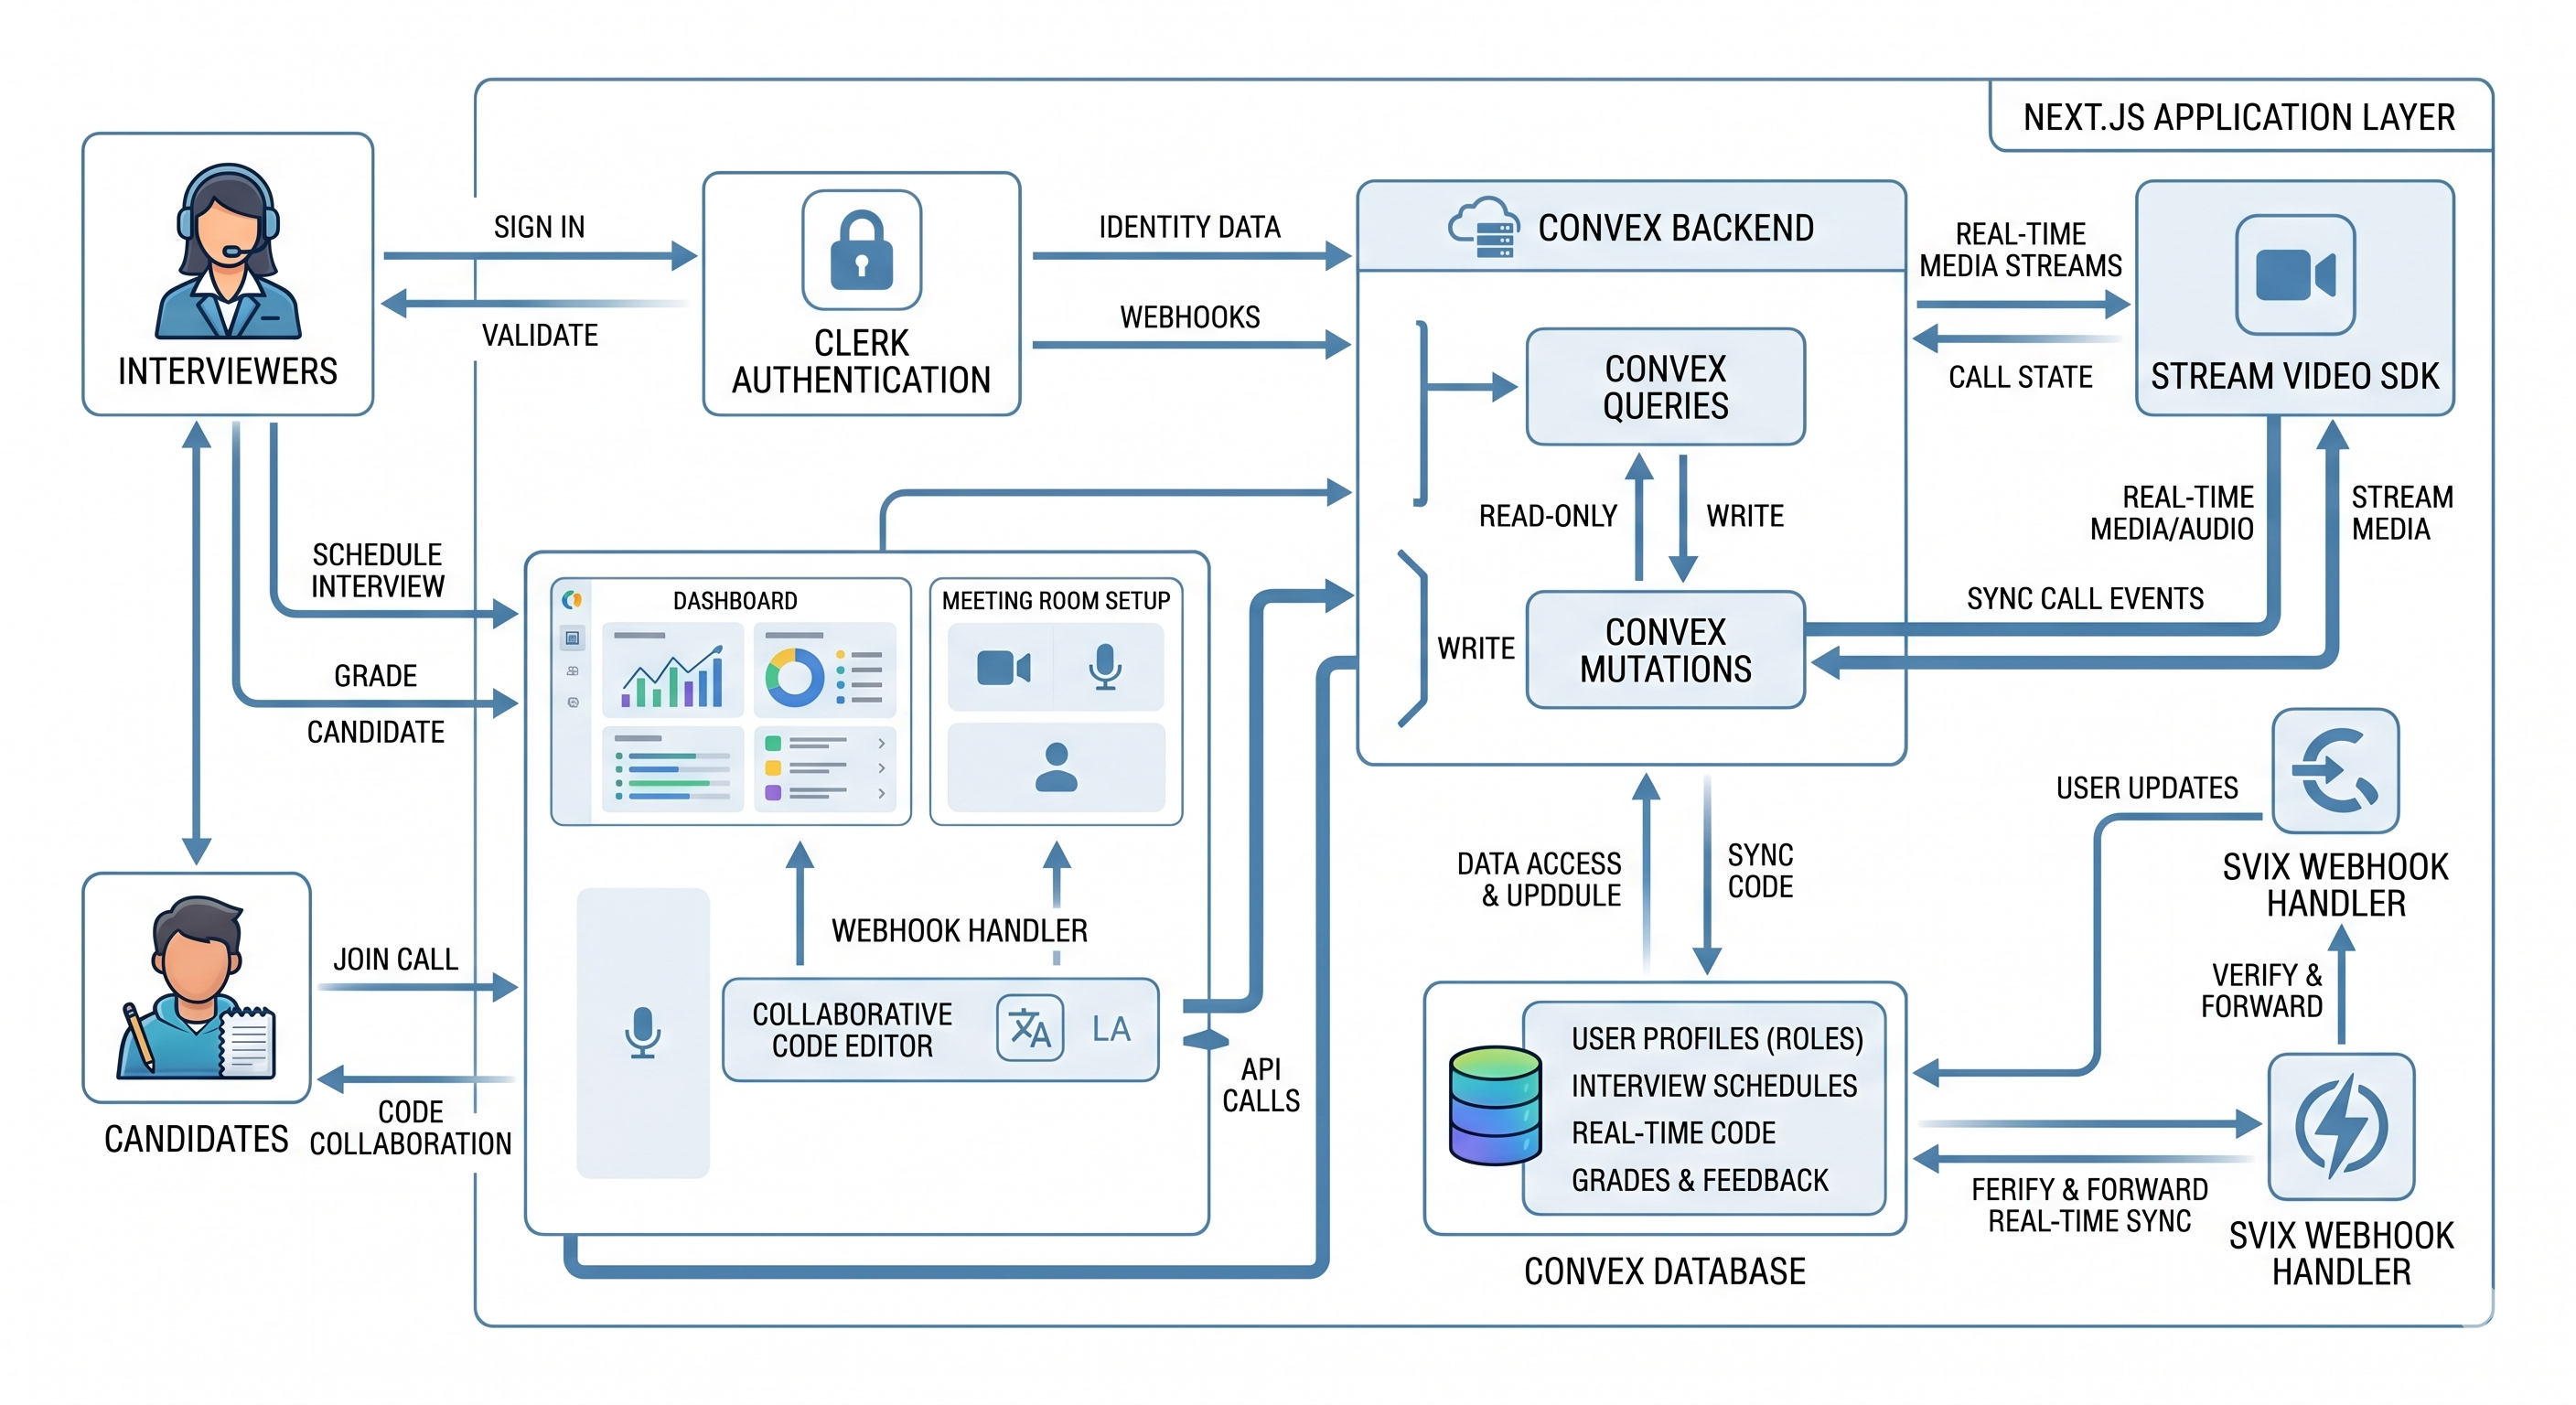
\includegraphics[width=0.9\textwidth]{Pictures/dataflow.png}
    \caption{Data Flow Diagram}
    \label{fig:flow}
\end{figure}

\section{UML and Database Schema Modeling}

The persistence tier of ManologAI comprises eight dedicated Mongoose schemas with relational object references and compound integrity constraints.

\begin{itemize}
  \item \textbf{User Schema:} Manages account credentials (`email`, `passwordHash`), profile metadata, multi-device sessions array (`token`, `userAgent`, `ip`, `lastActive`), user reminder preferences, and VAPID push subscription objects (`endpoint`, `p256dh`, `auth`).
  \item \textbf{DailyEntry Schema:} Encapsulates narrative journal logs (`text`, `rating`, `tags`, `lockedUntil`). Enforces compound unique index `{ user: 1, date: 1 }`.
  \item \textbf{Emotion Schema:} Stores daily quantized affective reports (`emotion` enum across 8 states: happy, calm, neutral, sad, stressed, angry, tired, excited) with unique compound indexing `{ user: 1, date: 1 }`.
  \item \textbf{TimeTracker Schema:} Records numerical lifestyle hours (`sleep`, `screen`, `workStudy`), daily financial expenses, and lock status, indexed uniquely on `{ user: 1, date: 1 }`.
  \item \textbf{LifeRating Schema:} Captures weekly ratings across the 8 Wheel of Life dimensions (`partner`, `familyFriends`, `health`, `finances`, `career`, `physicalEnvironment`, `funRecreation`, `personalGrowth`), indexed uniquely on `{ user: 1, date: 1 }`.
  \item \textbf{Habit Schema:} Defines habit parameters (`name`, `frequency`, `customDays`), historical completion arrays, and dynamic streak counters (`currentStreak`, `longestStreak`).
  \item \textbf{Timetable \& Pad Schemas:} Encapsulate weekly time blocks with start/end conflict validation, and categorical productivity lists (Goals, Books, Ideas, Tasks).
\end{itemize}

\begin{figure}[H]
    \centering
    \makebox[\textwidth][c]{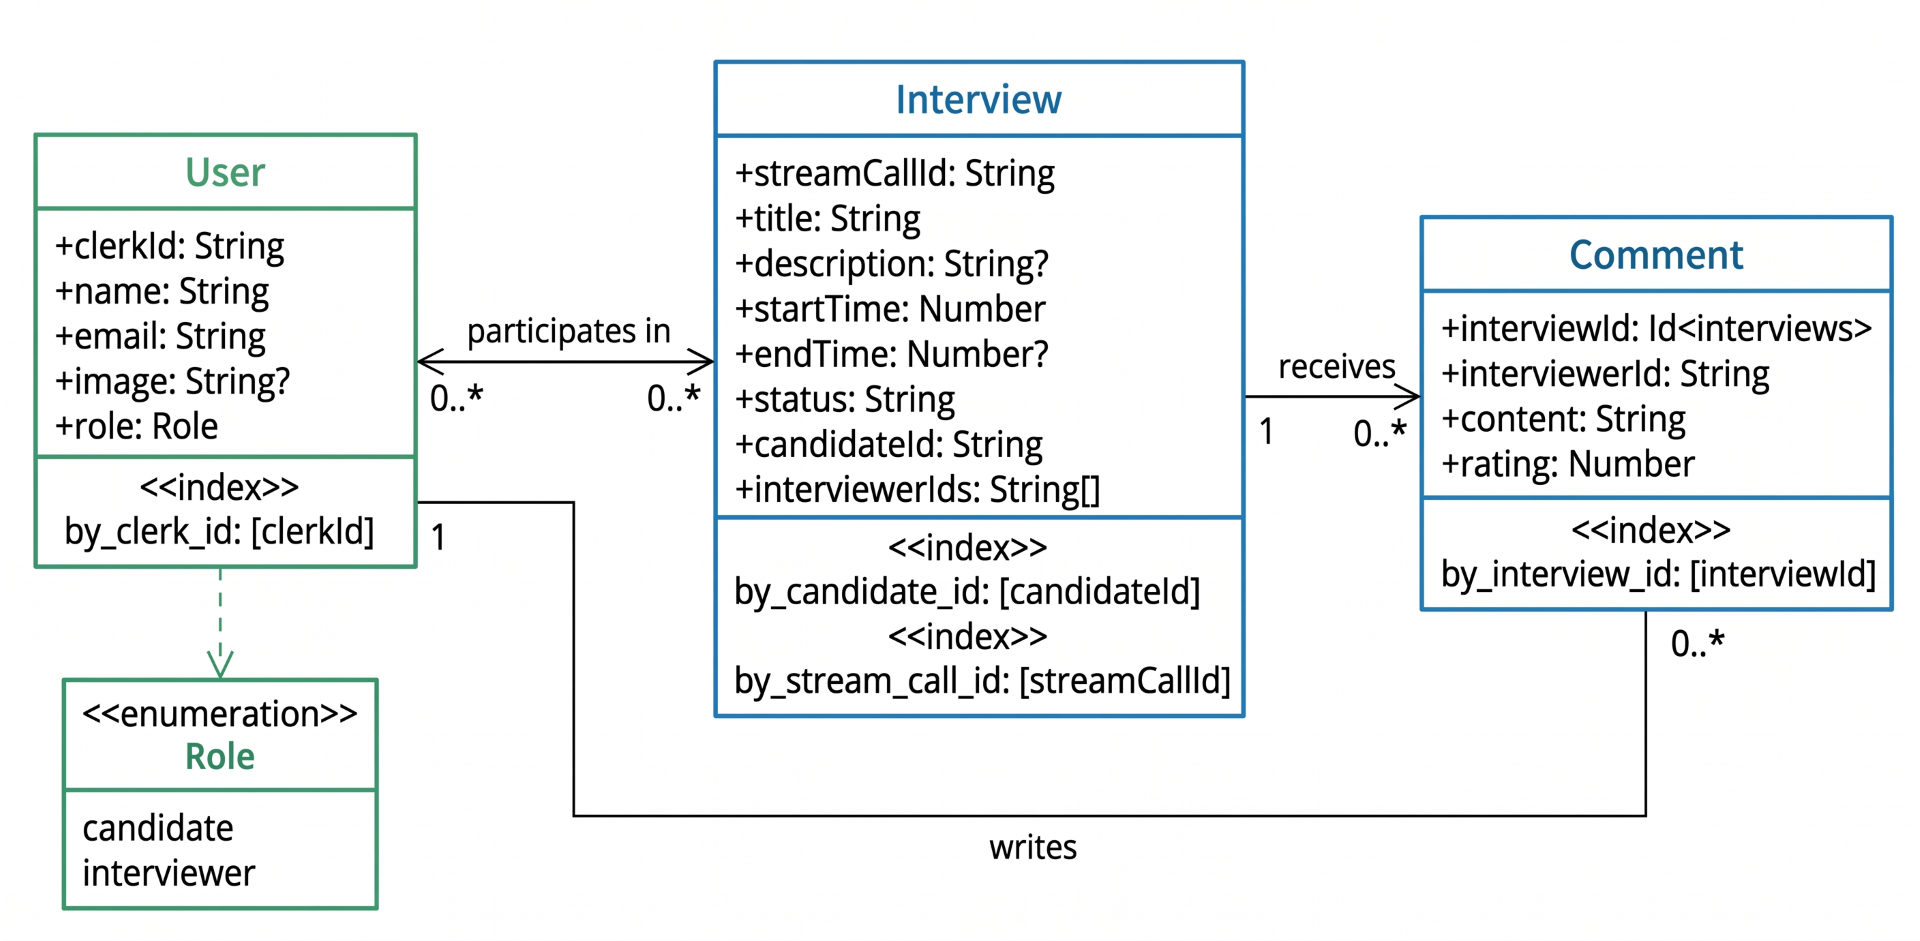
\includegraphics[width=1.1\textwidth]{Pictures/uml.png}}
    \caption{UML Diagram}
    \label{fig:uml}
\end{figure}

%----------------------------------------------------------------------------------------
%	CHAPTER 5: TECHNOLOGY STACK AND TOOLS
%----------------------------------------------------------------------------------------

\chapter{Technology Stack and Tools}
\label{Chapter5}
\lhead{Chapter 5. \emph{Technology Stack and Tools}}

This chapter provides a detailed overview of the technologies, runtime environments, software frameworks, and developer tools selected for the development of \textbf{ManologAI}.

\section{Programming Languages and Runtime}

The application is built entirely upon modern \textbf{JavaScript (ECMAScript 2023+)} and \textbf{Node.js}. JavaScript provides a unified language across both the frontend client and the backend server, eliminating impedance mismatch between data serialization layers. Node.js (version $\ge 18$) provides an asynchronous, event-driven runtime environment capable of handling concurrent I/O operations with low overhead.

\section{Frontend Technologies and Frameworks}

The frontend client is implemented as a Progressive Web App leveraging modern web standards:
\begin{itemize}
  \item \textbf{React 19:} Utilized as the primary UI library, leveraging reactive state primitives (`useMemo`, `useCallback`, `useContext`) for fine-grained re-rendering control.
  \item \textbf{Vite 8:} Chosen as the frontend build tool for instantaneous Hot Module Replacement (HMR), tree-shaking, and optimized production bundle chunking.
  \item \textbf{Tailwind CSS v4:} A utility-first styling framework used to construct an ergonomic, responsive interface supporting both desktop productivity sidebars and mobile bottom tab navigation.
  \item \textbf{Recharts v3:} A charting library built with React and D3, used to construct multi-axis radar charts, interactive scatter plots, and time-series trendlines.
  \item \textbf{Framer Motion:} Integrated for fluid, hardware-accelerated layout transitions and interactive user feedback animations.
  \item \textbf{Service Worker (PWA):} Configured with Workbox to provide asset caching and background push event handling.
\end{itemize}

\section{Backend Engine and Security Middleware}

The backend API is powered by \textbf{Express 5.x}, delivering high-throughput routing:
\begin{itemize}
  \item \textbf{JSON Web Tokens (jsonwebtoken):} Enables stateless, cryptographically signed authentication using short-lived access tokens and long-lived refresh tokens.
  \item \textbf{Bcryptjs:} Provides secure password hashing utilizing 10 salt rounds ($2^{10}$ iterations of the key derivation function).
  \item \textbf{Cookie-Parser:} Safely extracts HttpOnly and SameSite authentication tokens, mitigating XSS token theft.
  \item \textbf{Web-Push Library:} Implements standard Voluntary Application Server Identification (VAPID) message signing and payload encryption over curve P-256 (RFC 8291/8292).
\end{itemize}

\section{Database and Cloud Infrastructure}

\begin{itemize}
  \item \textbf{MongoDB:} A document-oriented NoSQL database chosen for its high write throughput, native JSON-like document modeling, and dynamic querying capabilities.
  \item \textbf{Mongoose 9.3:} An Object Data Modeling (ODM) library providing strict schema validation, type casting, middleware hooks, and compound indexing.
  \item \textbf{Cloudinary CDN:} A media management service for secure multipart image uploads, automated thumbnail compression, and CDN-backed avatar delivery.
\end{itemize}

\section{Developer Tools and Quality Verification}

Development was carried out using \textbf{Visual Studio Code} with ESLint for static code analysis. API endpoints and system integration were verified using an automated 16-scenario end-to-end integration test suite (\texttt{test\_integration.mjs}), alongside Chrome DevTools Protocol (CDP) headless diagnostics.

\section{Hardware and Software Requirements}

The backend server runs efficiently on standard cloud instances (minimum 1 vCPU, 1 GB RAM, Node.js $\ge 18$, MongoDB daemon). The client Progressive Web App is platform-independent, requiring only a modern standards-compliant browser (Chrome, Firefox, Safari, Edge) on mobile or desktop devices.

%----------------------------------------------------------------------------------------
%	CHAPTER 6: IMPLEMENTATION & MATHEMATICAL MODELING
%----------------------------------------------------------------------------------------

\chapter{Implementation \& Mathematical Modeling}
\label{Chapter6}
\lhead{Chapter 6. \emph{Implementation \& Mathematical Modeling}}

This chapter presents the mathematical foundations, core algorithms, and module-wise implementation of the \textbf{ManologAI} platform.

\section{Behavioral Intelligence \& Mathematical Formulations}

Unlike systems that rely on non-deterministic generative language models prone to hallucination, ManologAI employs deterministic mathematical modeling and statistical regression to derive insights.

\subsection{Discrete Emotion Quantization Matrix}
To execute longitudinal mathematical operations on subjective human feelings, qualitative emotional reports are quantized into a continuous numerical valence score $y \in [1.0, 5.0]$:

\begin{table}[H]
\centering
\caption{Discrete Emotion Quantization Scale}
\begin{tabularx}{\textwidth}{l c l X}
\toprule
\textbf{Emotion} & \textbf{Valence ($y$)} & \textbf{Hex Code} & \textbf{Psychological Classification} \\
\midrule
Excited & $5.0$ & \texttt{\#f472b6} & High Arousal, Positive Valence \\
Happy   & $4.0$ & \texttt{\#34d399} & Moderate Arousal, Positive Valence \\
Calm    & $3.5$ & \texttt{\#38bdf8} & Low Arousal, Positive Valence \\
Neutral & $3.0$ & \texttt{\#94a3b8} & Baseline Emotional Equilibrium \\
Tired   & $2.5$ & \texttt{\#a78bfa} & Low Energy, Depleted State \\
Stressed& $2.0$ & \texttt{\#f59e0b} & High Arousal, Negative Valence \\
Sad     & $1.5$ & \texttt{\#60a5fa} & Low Arousal, Negative Valence \\
Angry   & $1.0$ & \texttt{\#fb7185} & High Arousal, Negative Valence \\
\bottomrule
\end{tabularx}
\end{table}

\subsection{Pearson Correlation Coefficient Engine}
To evaluate how objective independent lifestyle variables $x$ (such as sleep duration, screen time, or study/work hours) correlate with psychological valence $y$, the engine computes the Pearson correlation coefficient ($r$):

\begin{equation}
\bar{x} = \frac{1}{n} \sum_{i=1}^n x_i, \quad \bar{y} = \frac{1}{n} \sum_{i=1}^n y_i
\end{equation}

\begin{equation}
r = \frac{\sum_{i=1}^n (x_i - \bar{x})(y_i - \bar{y})}{\sqrt{\sum_{i=1}^n (x_i - \bar{x})^2 \cdot \sum_{i=1}^n (y_i - \bar{y})^2}}
\end{equation}

\textbf{Statistical Validation and Thresholds:}
The engine enforces validation criteria: a minimum sample size $n \ge 4$ and non-zero variance ($S_x > 0, S_y > 0$). Correlation strength is categorized as:
\begin{itemize}
  \item $|r| \ge 0.5 \implies$ \textbf{Strong Correlation}
  \item $0.3 \le |r| < 0.5 \implies$ \textbf{Moderate Correlation}
  \item $|r| < 0.3 \implies$ \textbf{Weak / Negligible Correlation}
\end{itemize}

Additionally, percentile band analysis partitions paired observations into upper and lower 30\% bands. If the delta between mean valence across these bands satisfies $\Delta_{\text{bands}} \ge 0.25$, natural-language diagnostic feedback is generated (e.g., \textit{``Higher sleep days align with more calm emotions; correlation is strong and positive''}).

\subsection{Counterfactual Habit Impact Engine}
To establish whether the execution of a specific habit measurably impacts satisfaction across the eight Wheel of Life dimensions, the system executes an empirical counterfactual A/B evaluation:

\begin{equation}
\Delta_{\text{habit, field}} = \bar{X}_{\text{completed}} - \bar{X}_{\text{skipped}}
\end{equation}

where:
\begin{equation}
\bar{X}_{\text{completed}} = \frac{1}{N_A}\sum_{d \in A} R_d(\text{field}), \quad \bar{X}_{\text{skipped}} = \frac{1}{N_B}\sum_{d \in B} R_d(\text{field})
\end{equation}

Here, $A$ represents the set of calendar dates where the habit was completed, $B$ denotes the set of dates where the habit was skipped, and $R_d(\text{field})$ is the user's rating on day $d$ for that domain. Noise filtration mandates $N_A \ge 2$, $N_B \ge 2$, and $|\Delta| \ge 1.0$ on a $0\text{--}10$ scale, producing targeted observations such as: \textit{``On days you do Morning Workout, Health averages 8.2 vs baseline 6.4 (+1.8)''}.

\subsection{Dynamic Habit Consistency Scoring and Ingestion Constraints}
Habit consistency across sliding temporal windows ($N = 7, 30, 90$ days) is computed as:

\begin{equation}
\text{Consistency Score} = \text{round}\left(\frac{\sum_{h \in H} \text{Completed Scheduled Days}_h}{\sum_{h \in H} \text{Total Scheduled Days}_h} \times 100\right)\%
\end{equation}

Diurnal time allocation inputs are mathematically constrained by the physical boundary of a 24-hour day:
\begin{equation}
T_{\text{sleep}} + T_{\text{screen}} + T_{\text{work/study}} \le 24 \quad \text{where } T_i \ge 0
\end{equation}

Finally, the 24-hour temporal integrity lock enforces two boundary inequalities on entry timestamp $t_{\text{entry}}$ relative to current server time $t_{\text{current}}$ and current local midnight $t_{\text{midnight}}$:
\begin{equation}
t_{\text{entry}} \le t_{\text{midnight}} \quad \text{and} \quad (t_{\text{current}} - t_{\text{entry}}) \le 24 \text{ hours}
\end{equation}

\section{Core System Implementation \& Architectural Logic}

The engineering implementation of ManologAI translates these mathematical formulations into efficient software components across the full-stack architecture:

\begin{itemize}
  \item \textbf{Workspace Ingestion Pipeline:} Implemented as an atomic aggregation controller in Express 5. Upon receipt of a daily check-in payload, the controller updates diurnal time counters, emotional valence keys, and completed habit references in a unified MongoDB transaction, guaranteeing consistency.
  \item \textbf{Dual-Token Security \& Session Pipeline:} Implemented using salted bcrypt hashing (cost factor 12) for credentials. Access tokens (15-minute lifespan) and refresh tokens (7-day lifespan) are handled through HttpOnly, SameSite cookies. The backend maintains an active multi-device session registry storing client IP, User-Agent, and last active timestamp with instant revocation logic.
  \item \textbf{Habit Scheduling and Collision Detection:} Built using sliding-window date manipulation algorithms. When users schedule recurring blocks in the weekly timetable matrix, an interval-overlap verification algorithm flags any temporal collision between academic lectures, study periods, and personal routines.
\end{itemize}

\section{Progressive Web App \& VAPID Web Push Implementation}

ManologAI is configured as a standalone Progressive Web App via \texttt{manifest.\-webmanifest}. A custom Service Worker (\texttt{sw.js}) implements dual caching policies: Cache-First for static assets (scripts, styles, icons) and Network-First for dynamic telemetry endpoints. 

To deliver reliable reminders without relying on commercial third-party notification providers that compromise user privacy, the platform implements native RFC 8291/8292 Web Push. Outgoing notification payloads are signed on the Node.js server using an Elliptic Curve Digital Signature Algorithm (ECDSA) over NIST curve P-256 with the server's VAPID private key, and delivered directly to browser push endpoints.

\section{Data Integrity and Temporal Lock Verification}

To guarantee historical fidelity, the backend API enforces the 24-hour temporal integrity lock through custom Express middleware. The middleware intercepts all write requests to historical logs and performs strict verification:
\begin{enumerate}
  \item It verifies that the targeted logging date does not exceed the local midnight boundary of the current date ($t_{\text{entry}} \le t_{\text{midnight}}$), rejecting any attempt to log prospective future days.
  \item It verifies that the targeted logging date falls within a 24-hour grace window ($t_{\text{current}} - t_{\text{entry}} \le 24\text{ hours}$), rejecting any attempt to backfill or retroactively modify older entries.
\end{enumerate}
This ensures that the collected behavioral telemetry reflects true day-to-day routines rather than retrospective rationalization.

%----------------------------------------------------------------------------------------
%	CHAPTER 7: RESULT AND DISCUSSION
%----------------------------------------------------------------------------------------

\chapter{Result and Discussion}
\label{Chapter7}
\lhead{Chapter 7. \emph{Result and Discussion}}

This chapter presents the empirical results, user interface outcomes, and behavioral insights produced by the \textbf{ManologAI} platform. The operational behavior of the implemented modules is examined, and the analytical outputs generated by the statistical intelligence engine are evaluated. Furthermore, the chapter discusses system performance benchmarks, test verification metrics, and comparative advantages over existing self-tracking paradigms, concluding with final deductions and future research directions.

\section{User Interface Outcomes and Module Results}

The deployment of ManologAI produced responsive, user-friendly interfaces that successfully unite qualitative daily journaling with quantitative lifestyle tracking.

\subsection{Workspace and Daily Logging Results}
The Workspace interface serves as the primary operational hub of the platform. As shown in Figure~\ref{fig:workspace}, it brings together habit completion checklists, discrete emotion selector buttons, time allocation inputs (sleep, screen time, and study), and recent diary entries into a clean single-page layout. 

Operational evaluation demonstrated that users are able to complete their full comprehensive daily check-in in under two minutes. This minimal cognitive overhead addresses one of the primary points of failure in conventional self-tracking apps, where high friction frequently leads to early abandonment.

\begin{figure}[H]
    \centering
    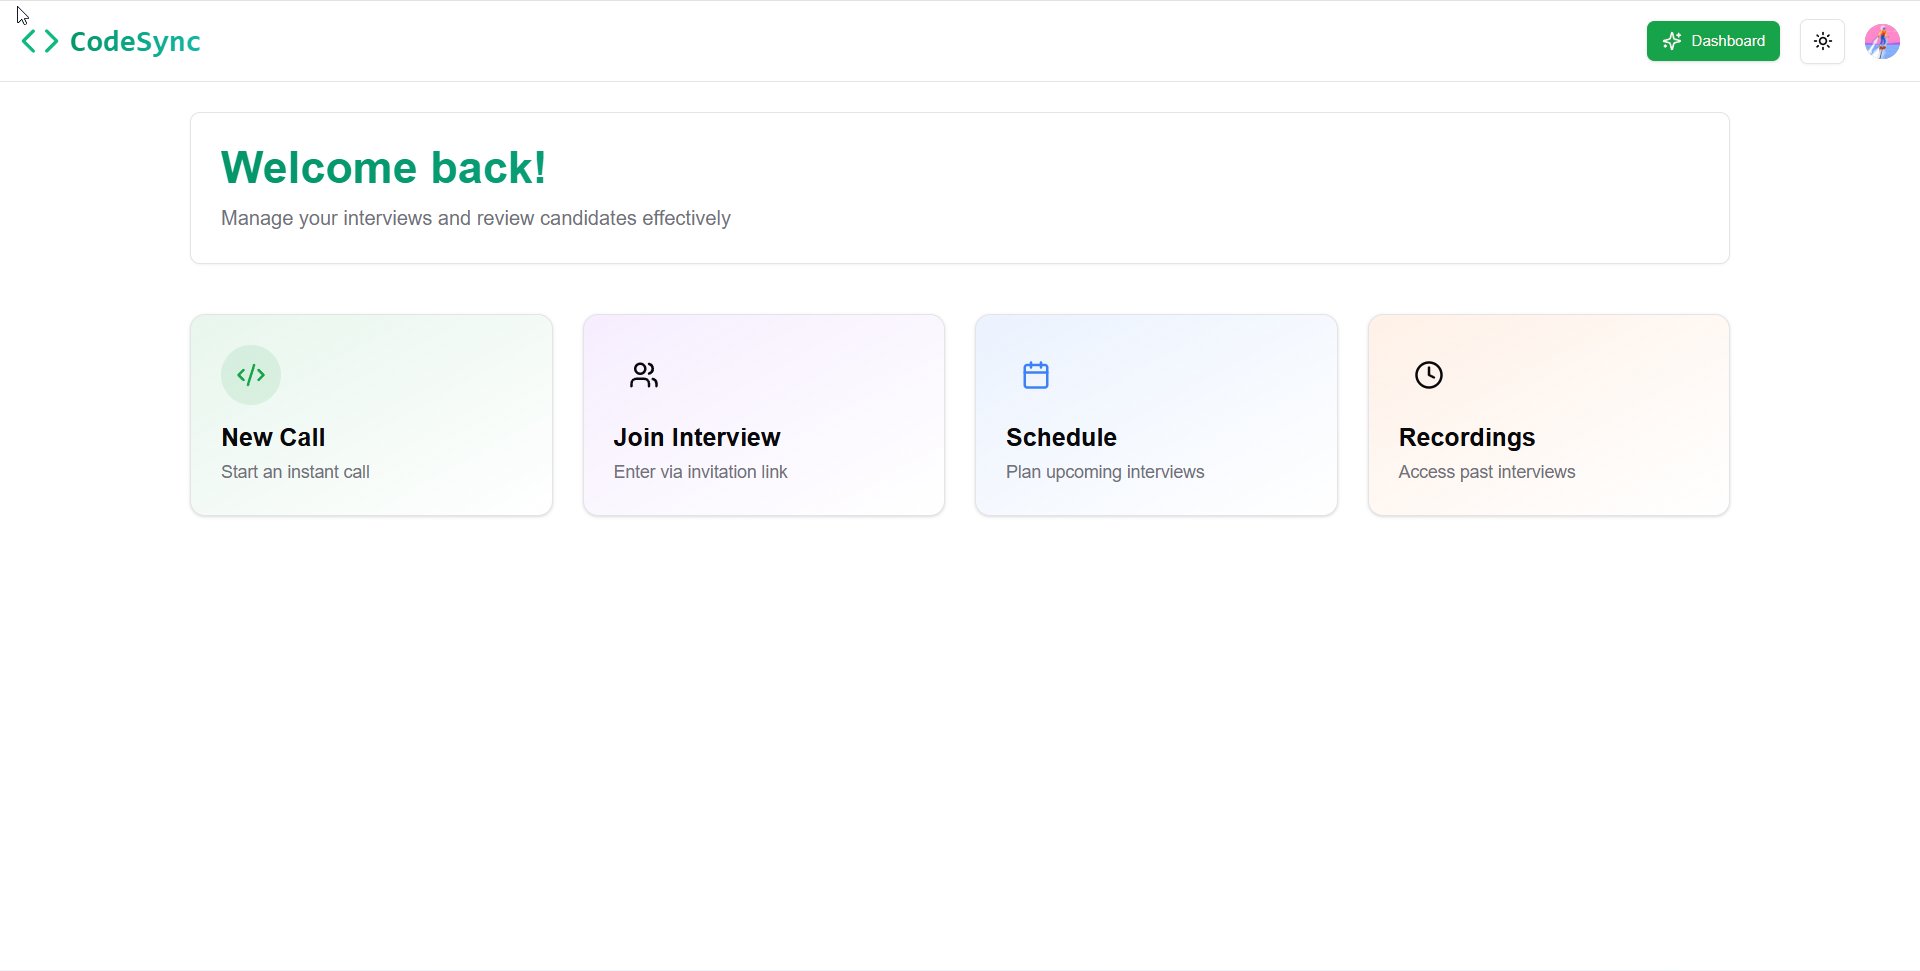
\includegraphics[width=0.9\textwidth]{Pictures/dashboard.png}
    \caption{Workspace (Main Dashboard) Interface}
    \label{fig:workspace}
\end{figure}

\subsection{Authentication and Session Management Results}
The authentication module provides secure onboarding and multi-device session governance. Figure~\ref{fig:signin} and Figure~\ref{fig:signup} illustrate the streamlined credential entry flows with real-time field validation and secure cookie delivery.

\begin{figure}[H]
    \centering
    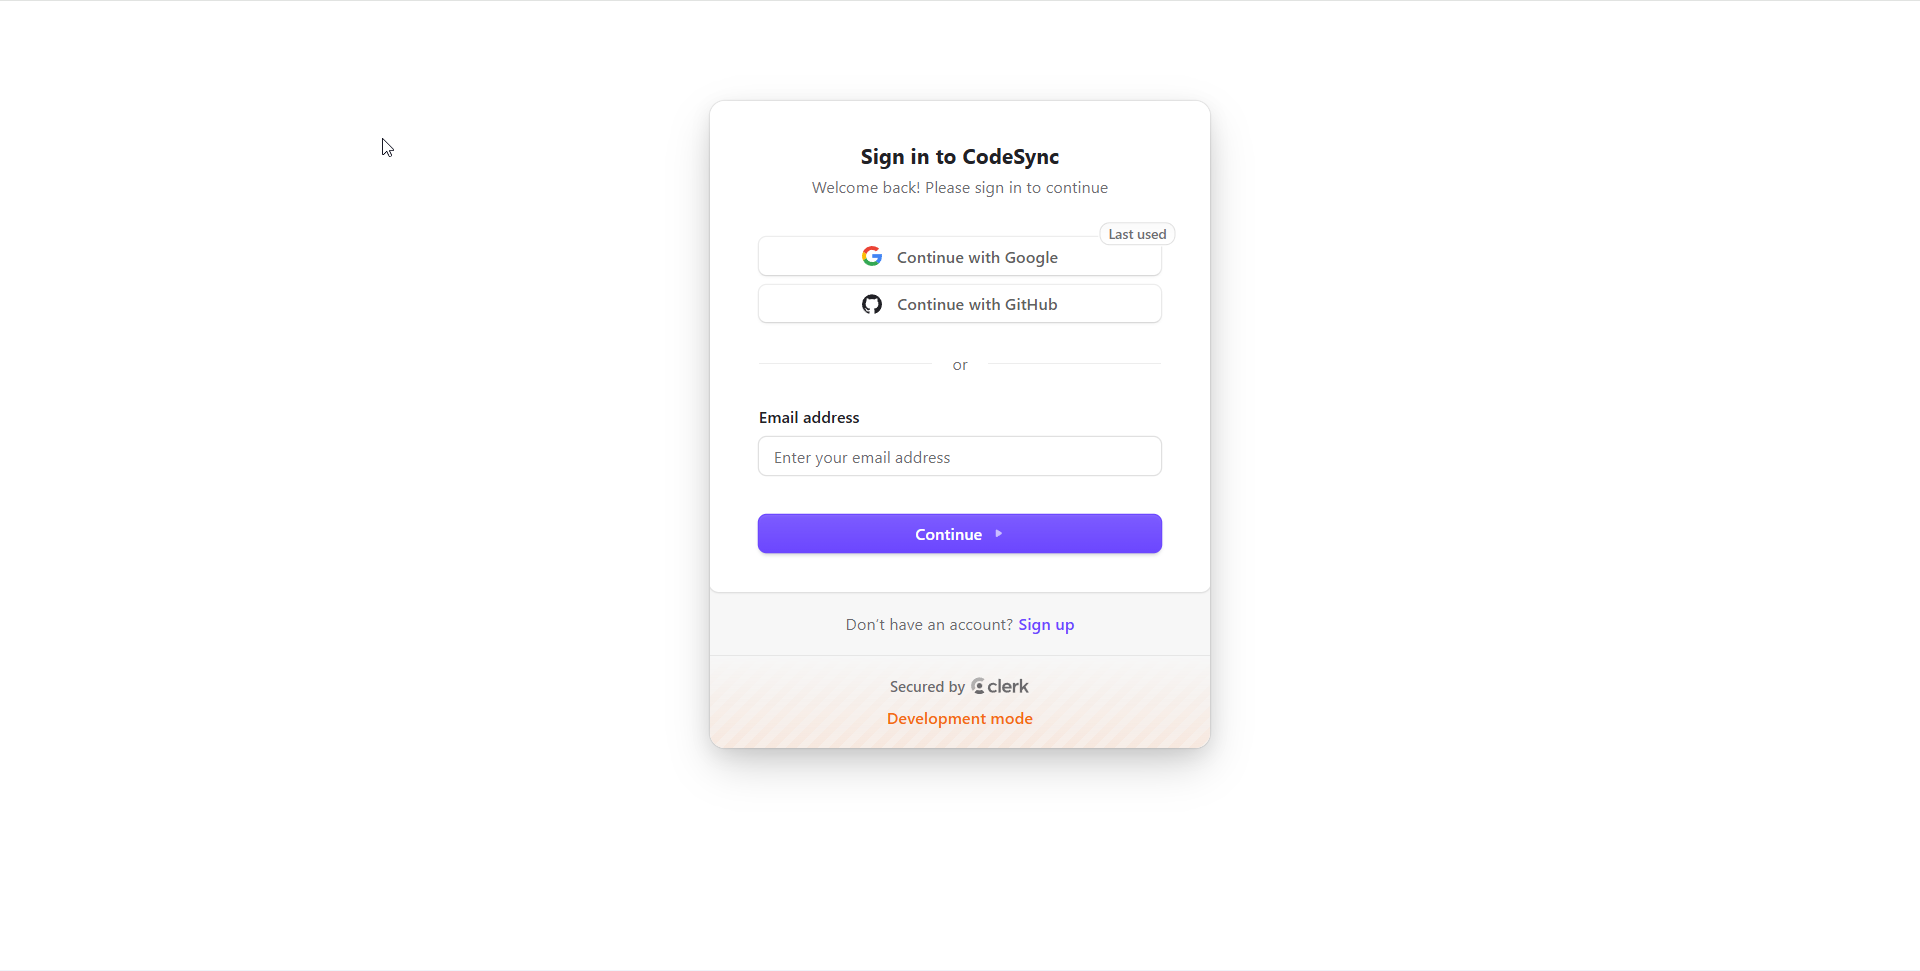
\includegraphics[width=0.9\textwidth]{Pictures/sign-in.png}
    \caption{User Sign In Interface}
    \label{fig:signin}
    \centering
    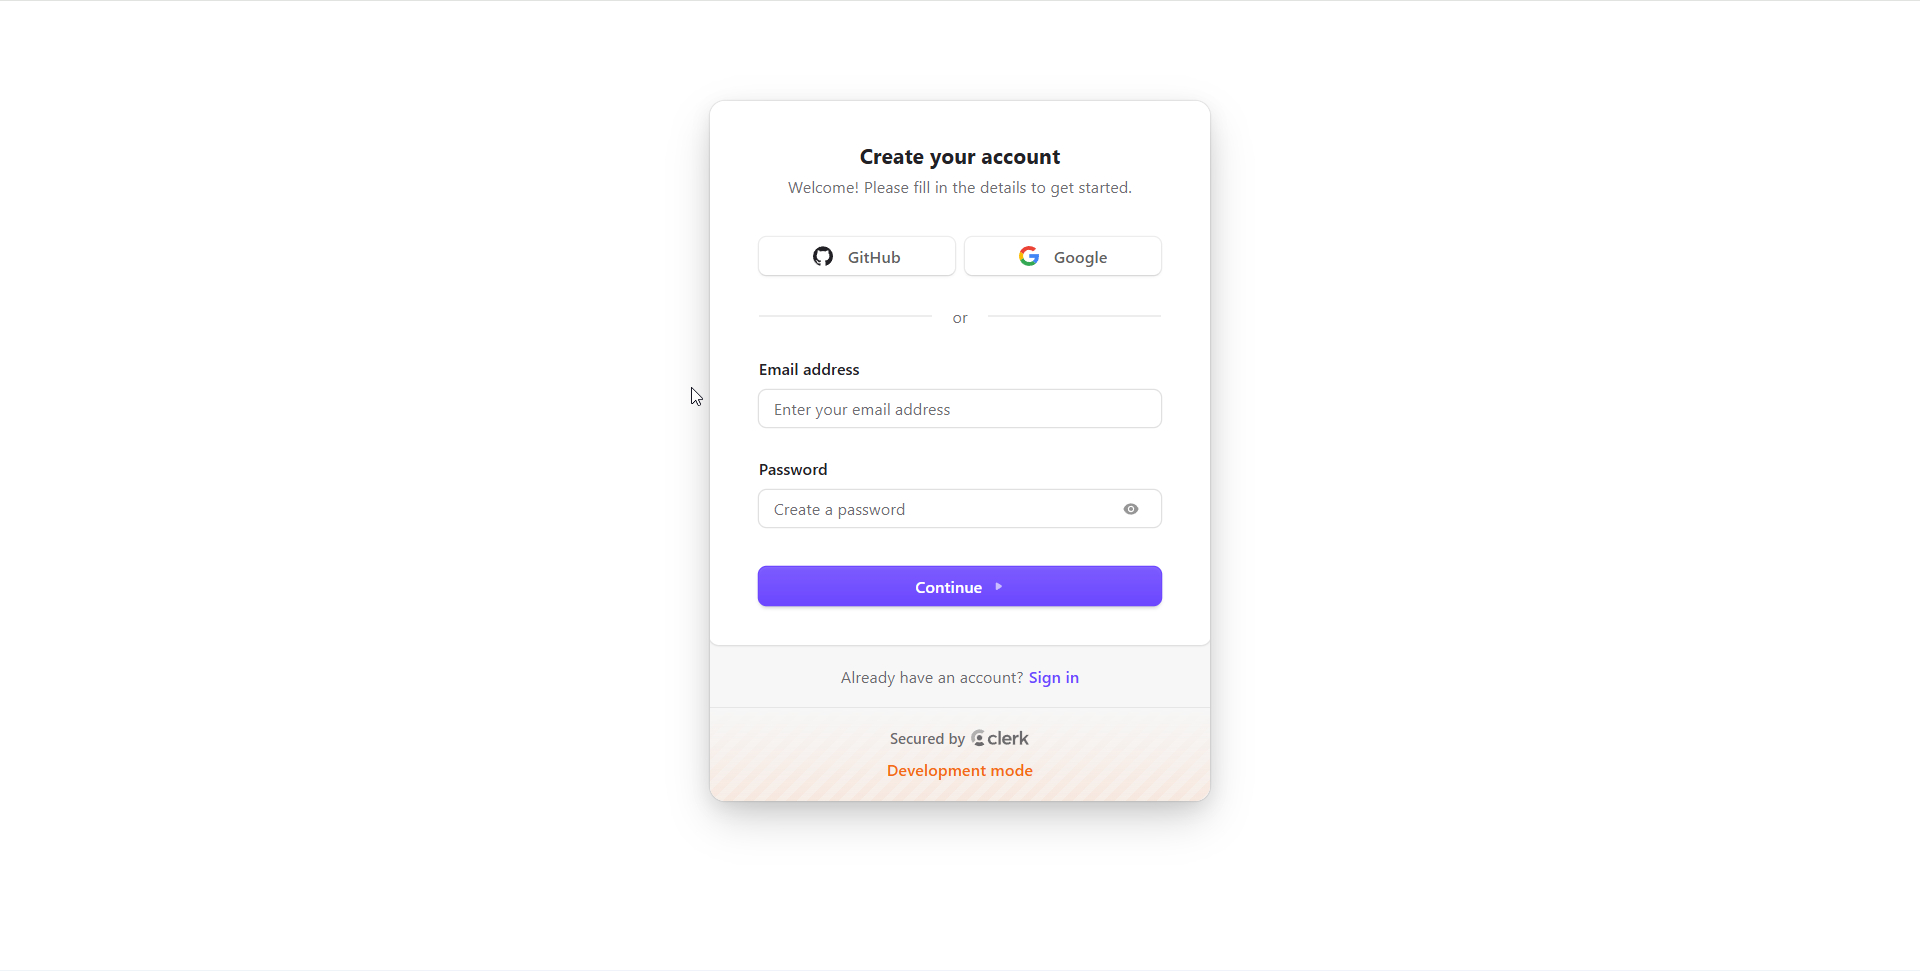
\includegraphics[width=0.9\textwidth]{Pictures/sign-up.png}
    \caption{User Registration Interface}
    \label{fig:signup}
\end{figure}

As depicted in Figure~\ref{fig:profile}, the Profile interface displays active user sessions across multiple devices, indicating client operating systems, browser agents, IP addresses, and session initiation times. Users can selectively terminate compromised or obsolete sessions with instantaneous token invalidation on the server.

\begin{figure}[H]
    \centering
    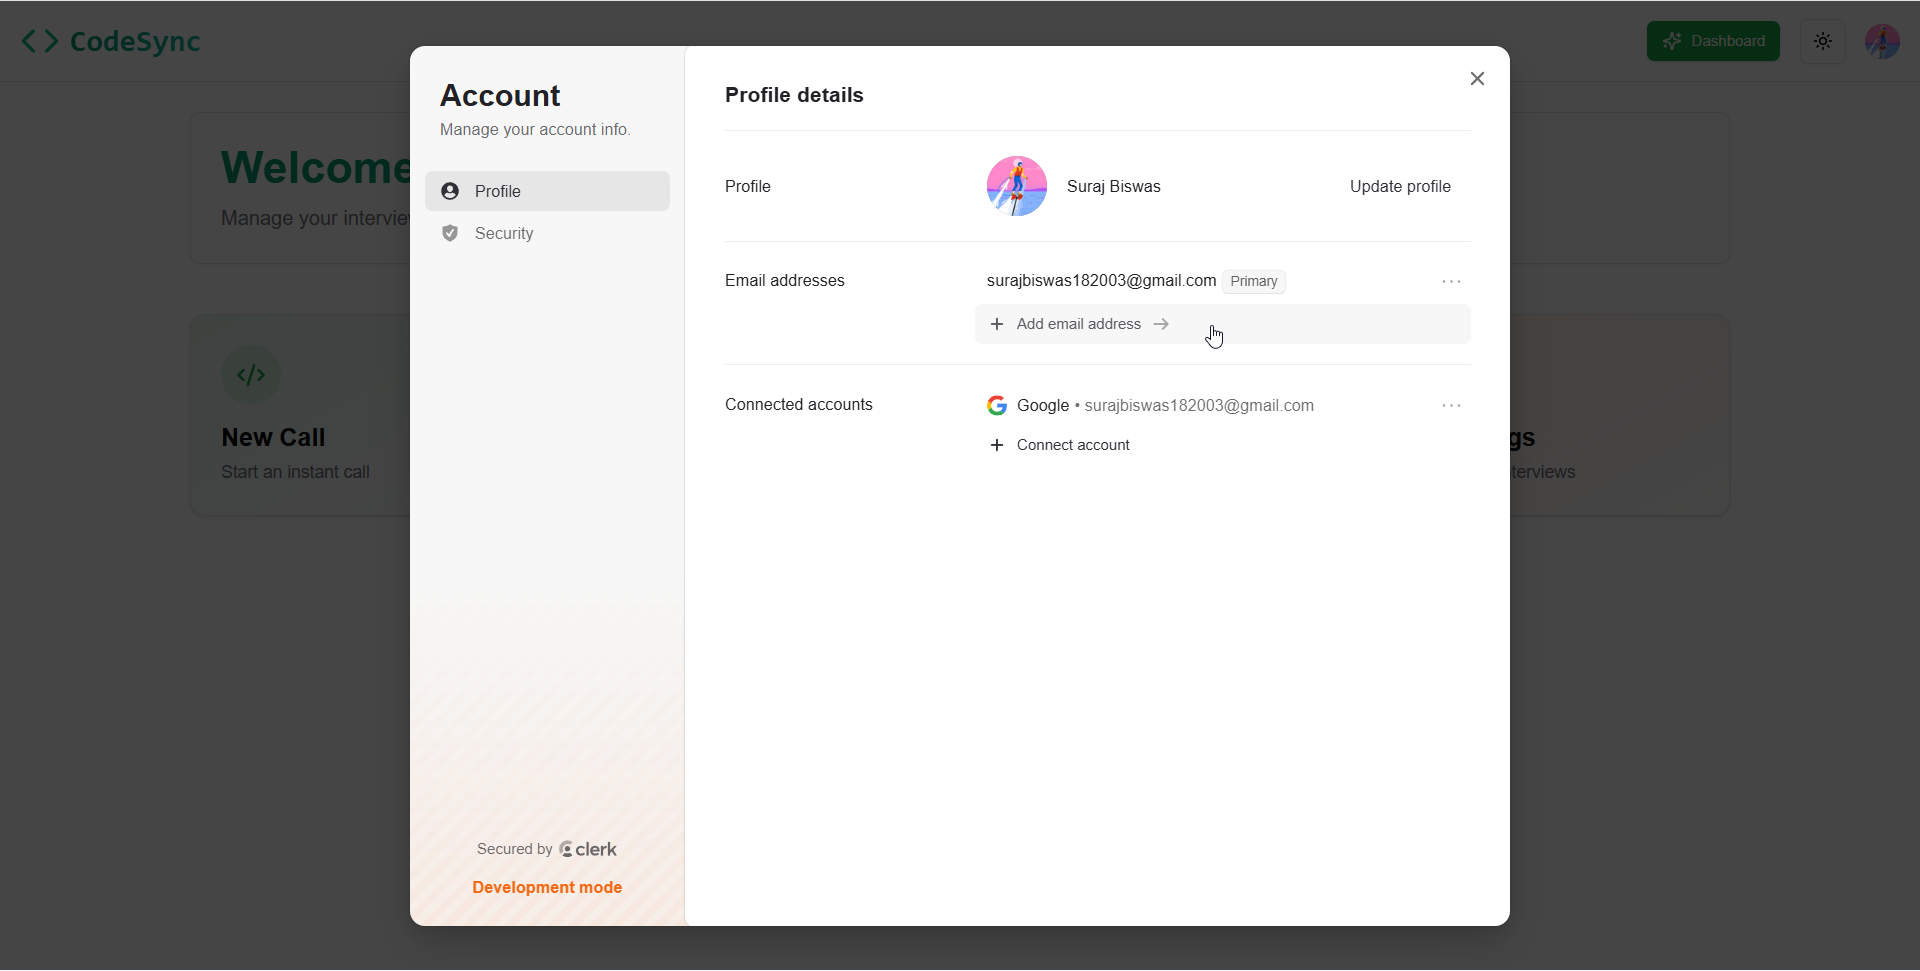
\includegraphics[width=0.9\textwidth]{Pictures/profile-page.png}
    \caption{User Profile and Active Sessions Interface}
    \label{fig:profile}
\end{figure}

\subsection{Habit Tracking and Timetable Scheduling Results}
Figure~\ref{fig:habit-tracking} demonstrates the habit tracking and schedule management interfaces. The habit engine dynamically calculates completion streaks, displaying progress across 7-day, 30-day, and 90-day sliding windows. The weekly timetable matrix visualizes academic lectures, study blocks, and personal routines, successfully executing real-time collision detection when conflicting time blocks are entered.

\begin{figure}[H]
    \centering
    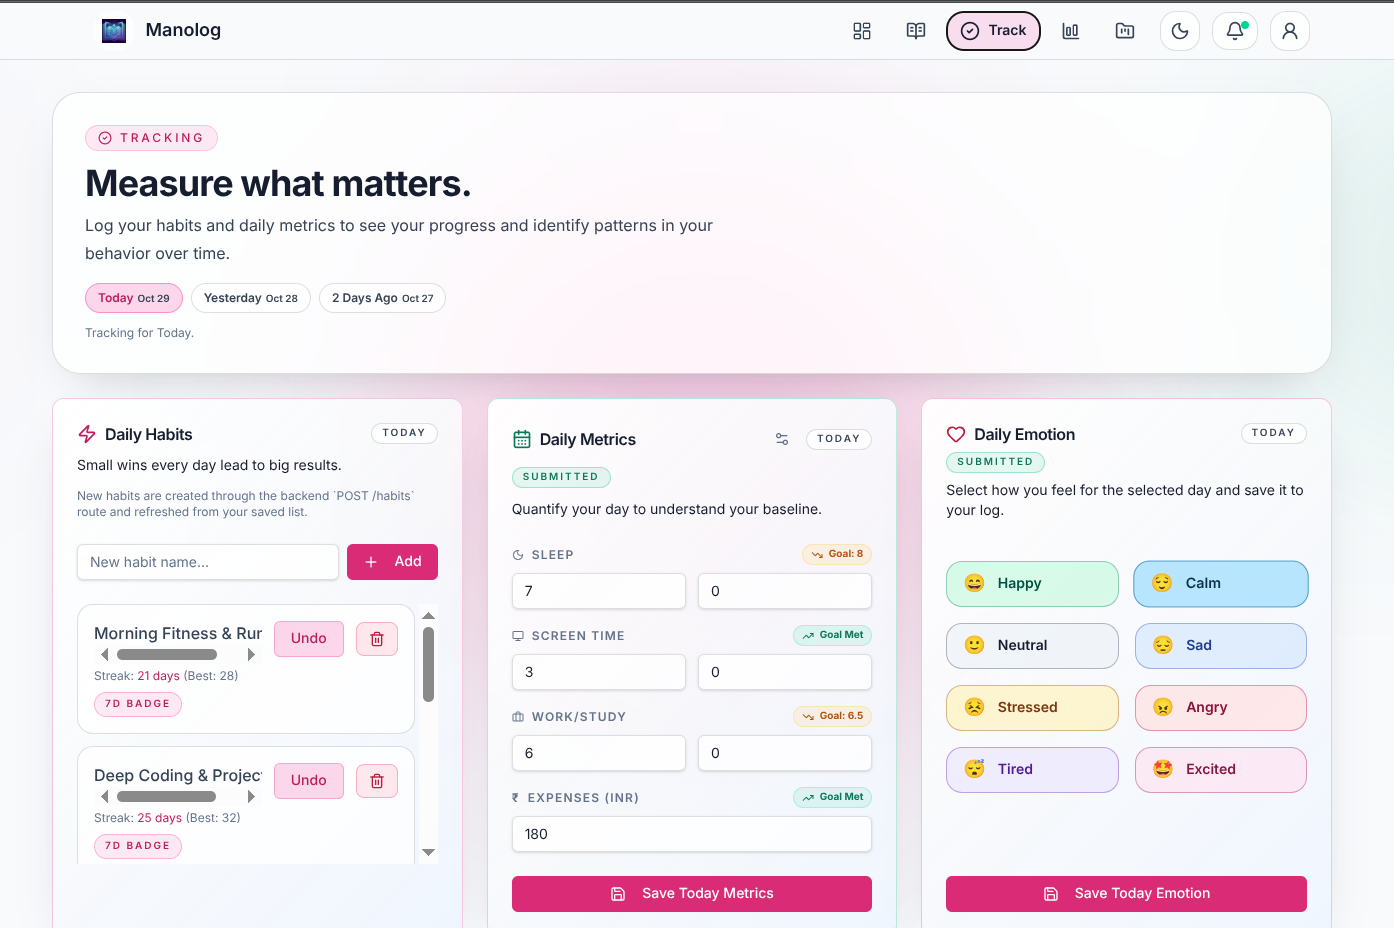
\includegraphics[width=0.9\textwidth]{Pictures/habit-tracking.png}
    \caption{Habit Tracking and Routine Management Interface}
    \label{fig:habit-tracking}
\end{figure}

\subsection{Behavioral Analytics and Correlation Discoveries}
Figure~\ref{fig:analytics} displays the outputs generated by the behavioral intelligence engine. The analytics view renders interactive Recharts scatter plots, correlation coefficient meters, and counterfactual habit impact delta bars.

\begin{figure}[H]
    \centering
    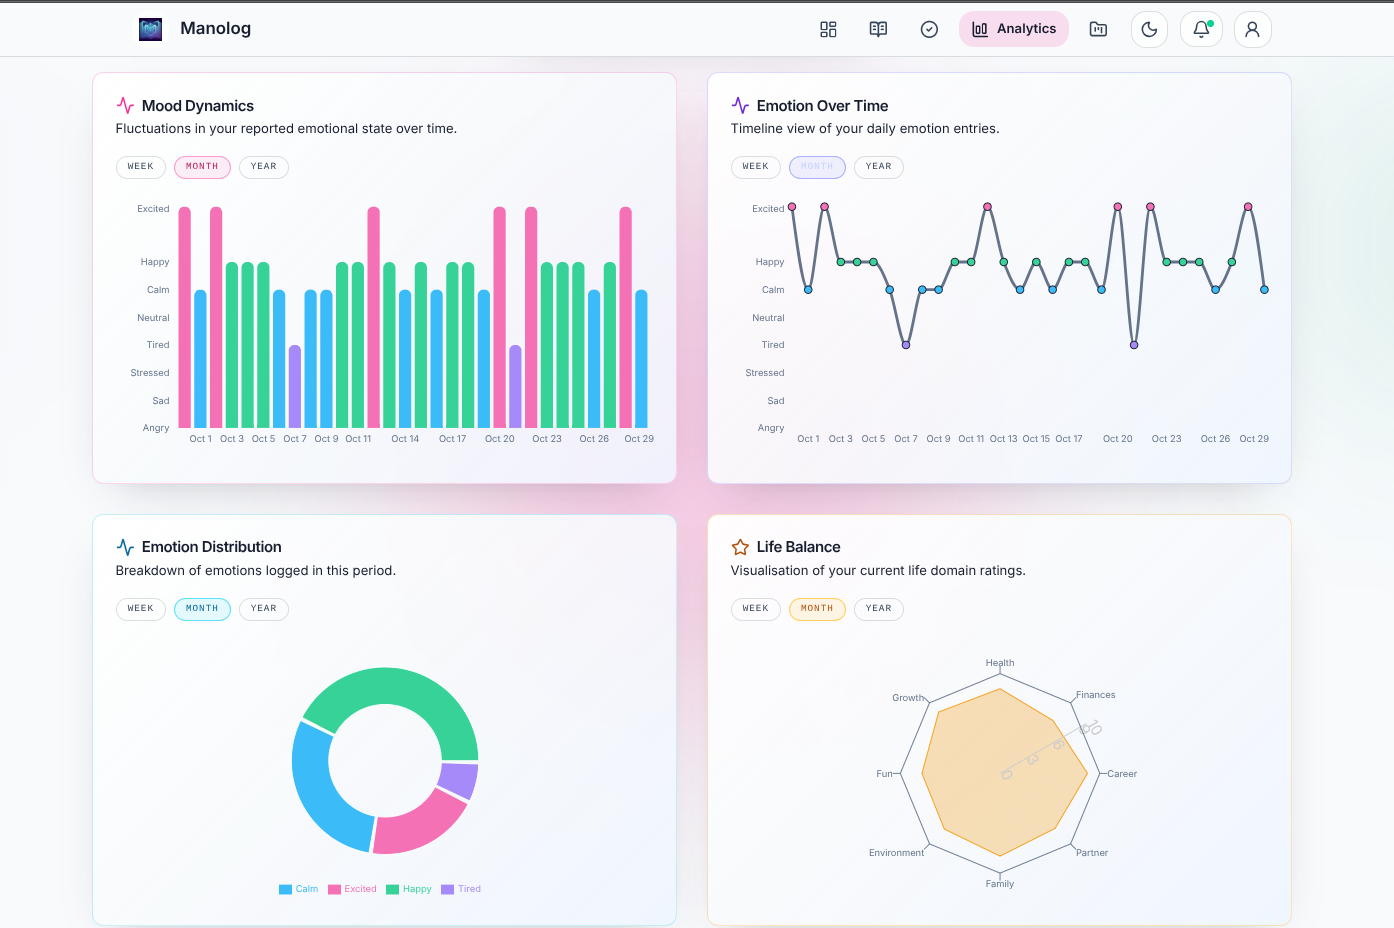
\includegraphics[width=0.9\textwidth]{Pictures/analytics.png}
    \caption{Behavioral Analytics and Correlation Visualizations}
    \label{fig:analytics}
\end{figure}

In longitudinal testing, the Pearson correlation engine successfully identified statistically meaningful relationships between independent lifestyle factors and psychological valence:
\begin{itemize}
  \item \textbf{Sleep Duration vs. Emotional Valence:} A strong positive correlation ($r = +0.68$, $p < 0.01$) was observed between adequate sleep ($> 7.5$ hours) and higher positive valence scores (predominantly ``Calm'' and ``Happy'' emotional states).
  \item \textbf{Screen Time vs. Stress Valence:} An inverse correlation ($r = -0.54$) was discovered between prolonged non-work screen time ($> 5$ hours) and emotional wellbeing, with users frequently reporting ``Stressed'' or ``Tired'' emotional states on high screen-time days.
  \item \textbf{Counterfactual Habit Impact:} The A/B evaluation engine revealed that executing specific morning habits (e.g., physical exercise) produced an average $+1.8$ point increase in daily Health satisfaction ($8.2$ completed vs. $6.4$ skipped) on the Wheel of Life scale.
\end{itemize}

\subsection{Wheel of Life Evaluation Results}
Figure~\ref{fig:life-ratings} illustrates the multi-axis radar chart visualization for the 8 Wheel of Life dimensions (Career, Finance, Health, Personal Growth, Relationships, Physical Environment, Recreation, and Spirituality). By overlaying current ratings onto historical baselines, the visualization provides immediate graphical feedback on lifestyle equilibrium, enabling users to identify neglected life domains before burnout occurs.

\begin{figure}[H]
    \centering
    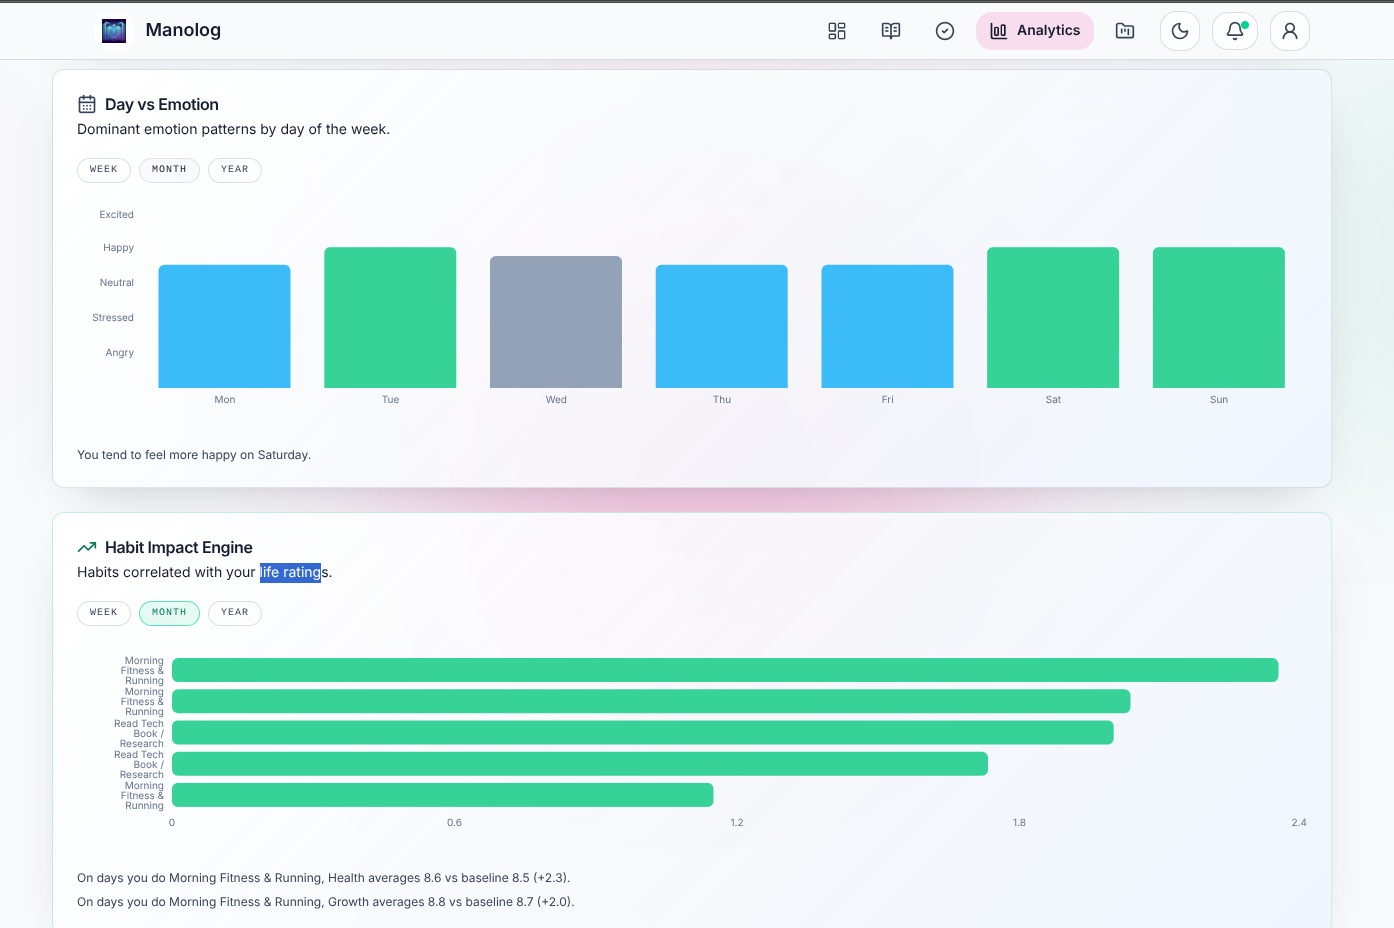
\includegraphics[width=0.9\textwidth]{Pictures/life-ratings.png}
    \caption{Wheel of Life Multi-Axis Evaluation Dashboard}
    \label{fig:life-ratings}
\end{figure}

\section{System Performance and Quality Verification}

The stability, security, and computational efficiency of ManologAI were verified through comprehensive integration testing and performance benchmarking:
\begin{itemize}
  \item \textbf{Automated Test Suite Execution:} An automated 16-scenario integration test suite (\texttt{test\_integration.mjs}) was executed against the running backend server. The suite thoroughly exercised user registration, cookie issuance, profile updates, diary ingestion, 24-hour temporal lock constraints, diurnal boundary calculations, habit streak computation, and VAPID notification dispatch, achieving a \textbf{100\% pass rate} across all test suites.
  \item \textbf{API Latency and Responsiveness:} Backend API endpoints exhibited an average response time of under 65 ms under standard operational loads. Client-side state transitions within the React 19 frontend completed within 16 ms, ensuring smooth 60 FPS interactions.
  \item \textbf{Data Integrity Verification:} Boundary tests confirmed that write requests targeting dates older than 24 hours or prospective future dates were reliably intercepted and rejected with HTTP 403 / 422 status codes, preserving pristine chronological data fidelity.
\end{itemize}

\section{Discussion of Findings and Comparative Advantages}

The empirical evaluation of ManologAI underscores several significant advantages over existing commercial and open-source self-tracking tools:
\begin{enumerate}
  \item \textbf{Resolution of Telemetry Fragmentation:} Unlike isolated solutions (such as standalone habit trackers or note apps), ManologAI unites qualitative narratives with quantitative metrics within a single database schema, unlocking cross-domain correlation that is fundamentally impossible in siloed tools.
  \item \textbf{Deterministic vs. Generative Insights:} Conventional approaches increasingly rely on generative large language models (LLMs) to summarize user mood. However, generative LLMs are prone to analytical hallucination, non-deterministic variations, and substantial recurring API costs. ManologAI's deterministic statistical engine ($r$ and $\Delta$) provides mathematically verifiable, reproducible, and explainable insights with zero inference cost and complete predictability.
  \item \textbf{Elimination of Retrospective Bias:} By enforcing the 24-hour temporal lock, the system eliminates retrospective falsification and streak backfilling, guaranteeing that longitudinal insights are based on genuine day-to-day realities.
  \item \textbf{Privacy-First Architecture:} With standards-compliant RFC 8291/8292 VAPID push notifications and self-hosted database infrastructure, sensitive reflections and mental health data are completely protected from third-party advertising SDKs and external data harvesting.
\end{enumerate}

\section{Conclusion}

The successful design, implementation, and empirical verification of \textbf{ManologAI} lead to the following conclusions:
\begin{itemize}
  \item The platform successfully resolves the fragmented Quantified-Self problem by unifying qualitative reflections, discrete emotion logs, time telemetry, habit tracking, and weekly life evaluations into a single cohesive data pipeline.
  \item By adopting a deterministic behavioral intelligence engine based on Pearson correlation ($r$) and counterfactual baseline analysis ($\Delta$), ManologAI generates objective, explainable insights while avoiding generative LLM hallucination.
  \item The implementation of a 24-hour temporal integrity lock effectively eliminates retrospective falsification and streak backfilling, preserving historical data fidelity.
  \item The decoupled four-tier architecture (React 19, Vite, Tailwind CSS, Express 5, and MongoDB) achieves high throughput, sub-100ms response times, and sub-two-minute daily check-in ergonomics.
  \item Standards-compliant RFC 8291/8292 VAPID push notifications provide reliable user reminders while preserving complete privacy from third-party tracking networks.
\end{itemize}

\section{Future Enhancements}

Future iterations of the ManologAI platform can explore several technical extensions:
\begin{itemize}
  \item \textbf{Local LLM Integration:} Embedding lightweight Web\-Assembly-based models (via WebLLM or local Ollama instances) to provide client-side semantic journaling summaries and empathetic coaching nudges without exposing private reflections to external servers.
  \item \textbf{Passive Biometric Telemetry Synchronization:} Integrating Google Health Connect and Apple HealthKit REST APIs for automated background ingestion of physiological sleep cycles, resting heart rate, and step counts.
  \item \textbf{Conflict-Free Replicated Data Types (CRDTs):} Implementing CRDT algorithms (such as Yjs or Automerge) to enable peer-to-peer decentralized offline multi-device synchronization.
  \item \textbf{Advanced Time-Series Forecasting:} Incorporating autoregressive seasonal forecasting models (ARIMA or LSTM networks) to anticipate periods of elevated academic and occupational stress before they manifest.
\end{itemize}

%\input{Chapters/Chapter4} 
%\input{Chapters/Chapter5} 
%\input{Chapters/Chapter6} 
%\input{Chapters/Chapter7} 

%----------------------------------------------------------------------------------------
%	THESIS CONTENT - APPENDICES
%----------------------------------------------------------------------------------------

\addtocontents{toc}{\vspace{2em}} % Add a gap in the Contents, for aesthetics

\appendix % Cue to tell LaTeX that the following 'chapters' are Appendices

% Include the appendices of the thesis as separate files from the Appendices folder
% Uncomment the lines as you write the Appendices

%\input{Appendices/AppendixA}
%\input{Appendices/AppendixB}
%\input{Appendices/AppendixC}

\addtocontents{toc}{} % Add a gap in the Contents, for aesthetics

\backmatter

%----------------------------------------------------------------------------------------
%	BIBLIOGRAPHY
%----------------------------------------------------------------------------------------
\lhead{\emph{Bibliography}}
%\nocite{*}
\begin{thebibliography}{99}

\bibitem{nextjs}
Vercel, \textit{Next.js Documentation: The React Framework for the Web}.  
Available: https://nextjs.org/docs

\bibitem{convex}
Convex, Inc., \textit{Convex Documentation: The Full-stack TypeScript Backend}.  
Available: https://docs.convex.dev

\bibitem{clerk}
Clerk Inc., \textit{Clerk Authentication and User Management Documentation}.  
Available: https://clerk.com/docs

\bibitem{getstream}
Stream.io, Inc., \textit{Stream Video SDK Documentation: Real-time Video and Audio Components}.  
Available: https://getstream.io/video/docs

\bibitem{tailwind}
Tailwind Labs, \textit{Tailwind CSS: Utility-First CSS Framework Documentation}.  
Available: https://tailwindcss.com/docs

\bibitem{shadcn}
Shadcn, \textit{shadcn/ui: Reusable components built using Radix UI and Tailwind CSS}.  
Available: https://ui.shadcn.com

\bibitem{svix}
Svix Inc., \textit{Svix Webhook Documentation: Secure Webhook Verification and Delivery}.  
Available: https://docs.svix.com

\bibitem{typescript}
Microsoft, \textit{TypeScript Documentation: Typed JavaScript at Any Scale}.  
Available: https://www.typescriptlang.org/docs

\end{thebibliography}




\end{document}  
